\chapter{Automatizált Internet mérő rendszer}
%(13-15 oldal): 

Jelen fejezet mutatja be az elkészült automatizált mérési rendszert, annak felépítését és működési elvét.

\section{Mérési elrendezés}
%(5 oldal): traceroute, iperf, mérési forgatókönyvek, PlanetLab

A felhőben vagy kliensen futó szoftver óránként felméri a PlanetLab hálózat gépeinek elérhetőségét és a kapott adatokat, statisztikákat eltárolja az adatbázisában. A PlanetLab hálózatában ugyanis elméleti szinten 1200 körüli végpont van, azonban ezeknek nagy százaléka elérhetetlen. A külön lépésben való feltérképezéssel rengeteg sikertelen kapcsolódást kerül el a mérőrendszer. A csatlakozásra képes célgépekre SSH kapcsolaton keresztül felcsatlakozik. Az egyes mérési forgatókönyveknek megfelelően parancssorozatokat futtat, majd azok eredményeit adatbázisban tárolja.
A nyers mérési eredmények, mint például a traceroute kimenet, később további feldolgozási lépéseken mennek keresztül. Végül az egyes kimutatásokhoz további statisztikák készülnek.
Az alábbiakban ezen lépések kerülnek részletesebb bemutatásra.

\subsection{A méréshez használt hálózat}

Az Interneten végzett mérésekhez szükséges a hálózatok különböző pontjain végezni méréseket. Egyes mérésekhez elegendő egy végpontból elvégezni a méréseket, azonban az csak lokális képet ad vissza, így torzítja az egész Internetről alkotott képet. A mérési rendszer üzemeltetéséhez ezért szükséges volt hozzáférést szerezni további a hálózatban résztvevő csomóponthoz. Így minél több résztvevő szolgáltat mérési adatokat, annál egységesebb képet tudunk kapni a kinyert adatokból. Az előző \ref{internet-measurement} szekcióban bemutatott hasonló mérési rendszerek szintén kiterjedt mérési hálózattal rendelkeztek. A PlanetLab hálózata kézenfekvő megoldás az Internetes mérések végzéséhez. Kiterjedésének nagysága biztosítja a mérés reprezentativitását, valamint megbízhatósága garantálja a mérések sikerességét.

A mérési rendszer azért jöhetett létre, mert a Budapesti Műszaki és Gazdaságtudományi Egyetem, ahol a Diplomamunkámat végeztem, résztvevője a PlanetLab szervezetnek. A részvételhez szükséges volt a megfelelő kapcsolattartó személyek kinevezése és a hálózat számára elérhetővé tenni két szerver gépet, amelyek megfelelnek a követelményeknek. A redundancia érdekében kötelező a két független gép. A hardveres paramétereken felül feltétel volt a szervezet által fejlesztett Linux disztribúció telepítése, amely fel van készítve a megfelelő virtualizáció támogatására. A tudományos mérések izolációjához szükséges a virtualizáció, így ha a szervezet egy résztvevője hibás programot futtat, az nem lesz kihatással a többiek által végzett mérésekre. A hozzáférések biztonságát a kötelező publikus-privát kulcsok használatával garantálják. Miután a mérésekhez generált publikus kulcs feltöltésre került a szervezet központi honlapjára, a mérésekhez már fel is lehetett használni.

A hálózatban elérhető gépekkel kapcsolatban fontos szempont továbbá, hogy hiába van elkülönített virtualizált környezet a résztvevők számára, azokon nem lehet tárolni adatokat. Bármikor felszólítás nélkül új virtualizált környezetet osztanak ki a felhasználók számára. Ezzel biztosítják a szerverek elérhetőségét és a folyamatos tisztulását. A Mérési rendszer készítésekor részben ezért volt szükséges az egyes mérési eredmények azonnali tárolása adatbázisban.

\subsection{Csatlakozás a hálózat számítógépeihez}

A mérések elvégzéséhez szükséges volt a PlanetLab hálózatának gépeihez való automatizált csatlakozás és parancs végrehajtás. A hálózatában résztvevő számítógépek listáját egy központi célgép szolgáltatja.

A mérések elvégzéséhez és feldolgozásához egységesen Python programozási nyelven megírt szkriptek lettek használva. A nyelv rugalmassága, támogatottsága és az elérhető könyvtárak bősége tette alkalmassá a gyors fejlesztésre. 
A méréseket végző program a Paramiko\cite{paramiko} könyvtárat használja az ssh kapcsolatok felépítéséhez és menedzseléséhez. A mérési kísérletek sok esetben hiúsultak meg különböző hibák, vagy a célszámítógép elérhetetlensége miatt, ezért ezen esetek kezelése fontos szempont volt a fejlesztés során. A \ref{fig:statistics} ábrákon látható statisztikák az első mérések adataiból készültek. A mérések óránként lettek elvégezve, lefutásonként 1354 csomóponthoz téve csatlakozási kísérletet. A vezérlő számítógép nem állandóan futott, így egy hónapban csak 23 nap készültek mérések, átlagosan 15 alkalommal.


\begin{figure}[h!]
\begin{center}
    \subfigure[Csatlakozási kísérletek eredményessége]{\label{fig:succeed}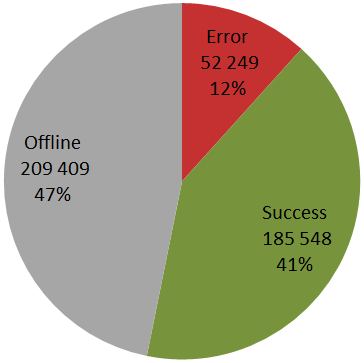
\includegraphics[scale=0.4]{figures/succeed.png}}
    \hspace{10mm}
    \subfigure[Hibák okai]{\label{fig:errors}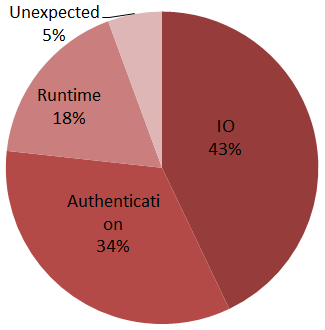
\includegraphics[scale=0.45]{figures/err.png}}
	\caption{Statisztikák\label{fig:statistics}}
\end{center}
\end{figure}

\subsection{Időzített mérési forgatókönyvek}
Az iperf mérések implementálásához új eljárás kidolgozására volt szükség a mérést menedzselő szoftverben. A korábbi traceroute mérések egyetlen parancs távoli futtatásából álltak, amelyek futási eredményét tároltuk el mérési eredményként. Az iperf és más sávszélesség mérő szoftverek működéséhez azonban szükséges mind egy adatcsomagokat küldő és egy adatcsomagokat fogadó példány futtatása a két különböző távoli gépen. Ennek lebonyolításához a mérést lebonyolító programnak több szálon kell futnia, a két távoli kódfuttatást egyszerre kell végeznie. Először az adatcsomagok fogadását (szerver oldal) végző programot kell elindítani, majd csak ezt követően lehet csak a mérést megkezdeni az adatcsomagokat küldő program (kliens oldal) elindításával. A mérést követően a szervert pedig le kell állítani. Ez a szituáció tovább bonyolódik, ha két sávszélesség mérést párhuzamosan szeretnénk végezni. Ez egy fennálló igény, mivel a későbbiekben az MPTCP\footnote{Multipath Transfer Protocol: Több párhuzamos TCP adatfolyamon végez kommunikációt a felsőbb rétegek felé egyetlen TCP kapcsolatot emulálva.} protokoll lehetséges viselkedését is vizsgálni szeretnénk.

Ezeket a lépéseket általánosítva olyan mérési forgatókönyvek létrehozását támogatja már a mérési rendszer, amely bármilyen távoli parancsok időzített futtatását garantálja. Ennek kialakítása a lehető legrugalmasabbra lett tervezve, amelynek működését a függelékben található példakód mutatja be. A kód egyszerűségének ellenére a mérés teljesen menedzselt, bármilyen hiba keletkezése le van kezelve és megfelelően naplózva és a mérési eredményben jelezve van. Garantálva van a helyes időzítés, a párhuzamos futás és a helyes leállás.

%A mérési forgatókönyvek rendkívül hasznosak, segítségükkel új mérések implementálása kényelmes és gyors.


\section{Geolokációs és AS információk}
Az internetes útvonalakat alkotó IP címekről több információt is tud kinyerni a mérési rendszer. Ilyen az ip címhez tartozó autonóm rendszer azonosítója, valamint a becsült geolokációs elhelyezkedése. Ezekhez Python szkriptek lettek készítve, amelyek ingyenes online szolgáltatásokat vesznek igénybe. A nagy feldolgozandó adatmennyiség és a sokszor lassú kapcsolódás miatt helyi gyorsítótár alkalmazása volt szükséges.

\section{Middlebox felderítés}
A tanszéken végzett Internetes kutatásokhoz hozzáadott értéket jelentett a mérési rendszer. A kutatás középpontjában napjaink egyik Internetes trendje az úgynevezett Middlebox-ok voltak. Ez egy általános fogalom minden olyan hálózati eszközre vonatkozóan, amely beavatkozik és manipulálja a rajta átmenő forgalmat. Ilyen lehet a hagyományos tűzfal vagy terheléselosztó, de manapság újabb és újabb célra használják fel, néha beavatkozva a végpontok közötti kapcsolatba. Ez az Internet alapjait jelentő protokollok működésére akár nem kívánt hatással is lehet, ezért fontos kutatási téma napjainkban.

A kutatáshoz való hozzájárulása a mérési rendszernek az interneten küldött csomagok TTL mezőjének a manipulációját vizsgálta. Egy célgépen a tcpdump nevű alkalmazást volt elindítva olyan beállításokkal, hogy csak a mérésben résztvevő csomagokat vizsgálja. A PlanetLab hálózat elérhető gépein pedig speciálisan elkészített csomagok voltak küldve a célgép felé a maximális 250-es TTL mezővel. A vizsgálat a Middlebox-ok TTL manipulációját figyelte a különböző csomagtípusokra vonatkozóan.

Három csomagtípus manipulációja volt vizsgálva:

\begin{itemize}
\item \textbf{ICMP Ping request} Hagyományos ping üzenet kérési csomagja
\item \textbf{TCP SYN port:22} TCP kapcsolatfelépítési csomag a 22-es portra, amely az ssh kapcsolatok fogadására szolgál
\item \textbf{TCP SYN port:80} TCP kapcsolatfelépítési csomag a 80-as portra, amely a http kapcsolatok fogadására szolgál
\end{itemize}

\pagebreak

A felhasznált parancsok a következők voltak:

\begin{lstlisting}[language=bash]
  # Celgepen futtatott parancs ICMP csomagok fogadasara
  sudo tcpdump -vnn -i eth0 icmp[icmptype] == 8 and dst host $ip
  # PlanetLab gepekrol kuldott ICMP csomagok parancsa
  ping -c 1 -t 250 $ip
  
  # A celgepen futtatott parancs TCP SYN csomagok fogadasara
  sudo tcpdump -vnn -i eth0 dst host $ip and "tcp[tcpflags] & (tcp-syn) != 0"
  # A PlanetLab gepeirol kuldott TCP csomagok parancsa
  nmap -v --ttl 250 --max-retries 1 -PS -p 80 $ip
  nmap -v --ttl 250 --max-retries 1 -PS -p 22 $ip
\end{lstlisting}


A mérés egy korábbi tanulmányt\cite{middlebox} vett alapul a felderítéshez. Az Internetes útvonalakon található, ttl mezőt manipuláló Middlebox-ok jelenlétét kimutatta a mérés. A mérés 75 szerverről küldött csomagok alapján lett elkészítve, mindegyik csomagtípusból egyet küldve a célgép felé, kivéve a 80-as portra küldöttek, amelyekből 3 csomag lett küldve gépenként.


\begin{figure}[!ht]
	\centering
	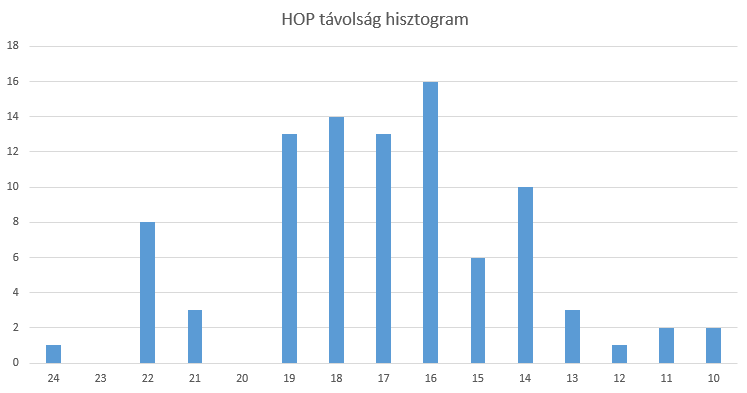
\includegraphics[width=0.5\textwidth, keepaspectratio]{figures/hop-hist.png}
	\caption{Az eredeti HOP távolsága a mért útvonalaknak}
	\label{fig:hop-hist}
\end{figure}


\begin{figure}[!ht]
	\centering
	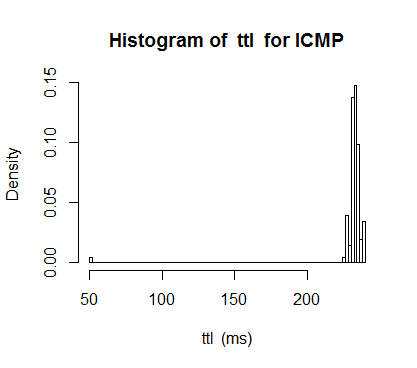
\includegraphics[width=0.3\textwidth, keepaspectratio]{figures/hist-ttl-icmp.png}
	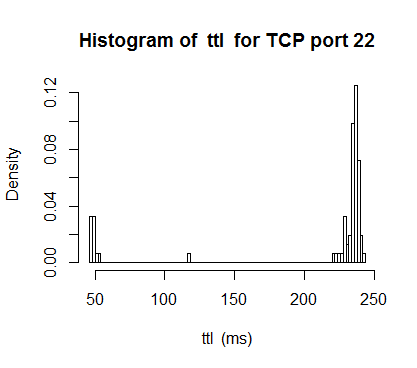
\includegraphics[width=0.3\textwidth, keepaspectratio]{figures/ttl-hist-22.png}
	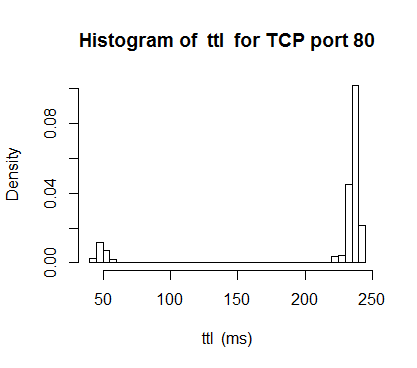
\includegraphics[width=0.3\textwidth, keepaspectratio]{figures/ttl-hist-port80.png}
	\caption{A fogadott csomagok TTL értékeinek előfordulási sűrűsége}
	\label{fig:ttl-hist}
\end{figure}

A \ref{fig:ttl-hist} ábrán látható, hogy az eredetileg 250-es TTL mezővel küldött csomagok egy része fogadáskor már egy közbülső elem által manipulálva lett. A manipuláció abból következtethető, hogy az útvonalak hosszúsága normális eloszlást követ, ahogy a \ref{fig:hop-hist} valamint függetlennek kellene lennie a csomag típusától.

Az ICMP csomagok ábráján egyetlen csomag érkezett vélhetően módosított TTL mezővel, későbbi ellenőrzéskor azonban kiderült, egy nem a mérésben résztvevő gép küldte. A méréshez használt csomagszűrő minden Ping requestet átengedett, azonban a mérés ideje alatt a colorado-i egyetem egyik szervere is küldött ilyen csomagot. Ilyen módon kimondhatjuk, hogy az ICMP csomagok TTL mezője nem megy keresztül módosításon. Ezzel szemben a TCP csomagok, amelyeket vizsgáltunk az esetek több mint 10\%-ában módosításon estek keresztül. A 80-as portra küldöttek 11\%-a, míg a 22-es portra küldöttek 15\%-a. Itt megjegyzendő, hogy nem következetes az útvonalakon közbeiktatott manipuláció. Egyes útvonalakon csak a 22-es portra küldött csomagok lettek változtatva, másokon csak a 80-as portra küldöttek és természetesen legtöbb esetben mindkettő. Ezen felül a 80-as portra küldött 3 csomagból, manipuláció esetén a legtöbb esetben egyszerre voltak csökkentett TTL mezőjűek és érintetlenek is.

Ez a mérés jól mutatja be a mérési rendszerben rejlő potenciált. A PlanetLab hálózatnak köszönhetően, az Internetre reprezentatív eredmények jöhetnek létre a gyorsan összeállítható mérési forgatókönyveknek hála.